\documentclass[12pt]{article}
  
  \usepackage[utf8]{inputenc}
  \usepackage[T1]{fontenc}
  \usepackage{geometry}
  \usepackage{graphicx}
  \geometry{a4paper}
  
  \usepackage[frenchb]{babel}
  
  \title{Assignment No. B11}
  \author{Roll no : 4430}
  \date{}
  
  \begin{document}
  \maketitle
  
\section{Problem Definition}
Implement Decision trees on Digital Library Data to mirror more titles(PDF) in the library application, compare it with Naive Bayes algorithm

\section{Learning Objectives}

\begin{enumerate}
\item To understand classification technique.
\item To learn Naive Bayes algorithm to efficiently classify tuples in database.
\end{enumerate}



\section{Mathematical Model}
Let S be the system of soluion of given problem statement.\\
s=\{s,e,I,O,F,DD,NDD,Su,Fu \}\\
where,\\
s=start state ;\\
such that, s=\{ \}\\
e=end state;\\
I =  represents set of input\\
I = \{d,m\}\\
where d is a det of tuples and m is a set of output classes\\
O represents set of output\\
O = Whether d $\in$ X also $\in$ m\\
F=set of functions.\\
F=\{f1,f2\}\\
where,\\
f1= Decision Tree Classifier\\
f1:X$\rightarrow$Y\\
such that X is the input set and Y is the decision tree.\\
f2= Naive Bayes classifier\\
f2:X$\rightarrow$Y\\
where X is the input and Y is the probability that X $\in$ m
DD = Deterministic Data\\
Input set is deterministic\\
NDD (Non Deterministic Data)\\
Decision Tree is non deterministic\\
Sc =Success case\\Input is classified correctly\\
Fc = Failure Case\\Wrong classification\\

\section{Theory}
\subsection{Decision tree}
A flow-chart-like tree structure\\
Internal node denotes a test on an attribute\\
Branch represents an outcome of the test\\
Leaf nodes represent class labels or class\\ distribution\\
Decision tree generation consists of two phases\\
Tree construction\\
At start, all the training examples are at the root\\
Partition examples recursively based on selected attributes\\
Tree pruning\\
Identify and remove branches that reflect noise or outliers\\

\subsection{Naive Bayes Classification}
The Bayesian Classification represents a supervised learning method as well as a statistical method for classification. Assumes an underlying probabilistic model and it allows us to capture uncertainty about the model in a principled way by determining probabilities of the outcomes. It can solve diagnostic and predictive problems.\\ 
Bayesian classification provides practical learning algorithms and prior knowledge and observed data can be combined. Bayesian Classification provides a useful perspective for understanding and evaluating many learning algorithms. It calculates explicit probabilities for hypothesis and it is robust to noise in input data.\\




\section{State Diagram }
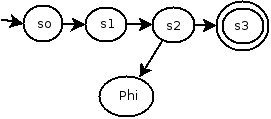
\includegraphics[scale=0.9]{state.png}\\
where,\\
so : Start state\\
s1 : Input state\\
s2 : Build Decision tree/Naive bayes classifier\\
s3 : End State = Result Displayed\\\\
phi : Failure Case\\

\section{Program Code and Output}
\begin{verbatim}
import java.io.*;

class DecisionTreeApp {
static BufferedReader keyboardInput = new
BufferedReader(new InputStreamReader(System.in));
static DecisionTree newTree;
public static void main(String[] args) throws IOException {
 // Create instance of class DecisionTree
        newTree = new DecisionTree();
      // Generate tree
        generateTree();
        // Output tree
        System.out.println("\nOUTPUT DECISION TREE");
        System.out.println("====================");
        newTree.outputBinTree();
        // Query tree
        queryTree();
        }

    /* GENERATE TREE */

    static void generateTree() {
        System.out.println("\nGENERATE DECISION TREE");
        System.out.println("======================");
        newTree.createRoot(1,"Semisterwise Computer Branch Subject");
        newTree.addYesNode(1,2,"Semister-1?");
        newTree.addNoNode(1,3,"Semister-2?");
        newTree.addYesNode(2,4,"Elective");
     	newTree.addYesNode(4,8," Subject is DMT");
    	newTree.addNoNode(4,9,"Subject is PC");
    	newTree.addNoNode(2,5,"Compulsory Subject");
    //  newTree.addYesNode(5,10,"Subject is SSDA");
        newTree.addYesNode(5,10,"Subject is PMCD");
    	newTree.addNoNode(5,11,"Subject is DAA");
        newTree.addYesNode(3,6,"Elective");
    	newTree.addYesNode(6,12,"Elective-1");
    	newTree.addNoNode(6,13,"Elective-2");
        newTree.addNoNode(3,7,"Compulsory Subject");
    	newTree.addYesNode(7,14,"Subject is SDMT");
    	newTree.addNoNode(7,15,"Subject is HPC");
        }

    /* QUERY TREE */
    
    static void queryTree() throws IOException {
        System.out.println("\nQUERY DECISION TREE");
        System.out.println("===================");
        newTree.queryBinTree();

        // Option to exit

        optionToExit();
        }

    /* OPTION TO EXIT PROGRAM */

    static void optionToExit() throws IOException {
        System.out.println("Exit? (enter \"Yes\" or \"No\")");
        String answer = keyboardInput.readLine();
        if (answer.equals("Yes")) return;
        else {
            if (answer.equals("No")) queryTree();
            else {
                System.out.println("ERROR: Must answer \"Yes\" or \"No\"");
                optionToExit();
                }
            }
        }
    }
    
//Output
ameeth@ubuntu-16.0.4:~/CL1$  javac DecisionTreeApp.java 
ameeth@ubuntu-16.0.4:~/CL1$  java DecisionTreeApp 

GENERATE DECISION TREE
======================
Created root node 1
Added node 2 onto "yes" branch of node 1
Added node 3 onto "no" branch of node 1
Added node 4 onto "yes" branch of node 2
Added node 8 onto "yes" branch of node 4
Added node 9 onto "no" branch of node 4
Added node 5 onto "no" branch of node 2
Added node 10 onto "yes" branch of node 5
Added node 11 onto "no" branch of node 5
Added node 6 onto "yes" branch of node 3
Added node 12 onto "yes" branch of node 6
Added node 13 onto "no" branch of node 6
Added node 7 onto "no" branch of node 3
Added node 14 onto "yes" branch of node 7
Added node 15 onto "no" branch of node 7

OUTPUT DECISION TREE
====================
[1] nodeID = 1, question/answer = Branch Computer
[1.1] nodeID = 2, question/answer = Semister-1?
[1.1.1] nodeID = 4, question/answer = Elective
[1.1.1.1] nodeID = 8, question/answer =  Subject is DMT
[1.1.1.2] nodeID = 9, question/answer = Subject is PC
[1.1.2] nodeID = 5, question/answer = Compulsory Subject
[1.1.2.1] nodeID = 10, question/answer = Subject is PMCD
[1.1.2.2] nodeID = 11, question/answer = Subject is DAA
[1.2] nodeID = 3, question/answer = Semister-2?
[1.2.1] nodeID = 6, question/answer = Elective
[1.2.1.1] nodeID = 12, question/answer = Elective-1
[1.2.1.2] nodeID = 13, question/answer = Elective-2
[1.2.2] nodeID = 7, question/answer = Compulsory Subject
[1.2.2.1] nodeID = 14, question/answer = Subject is SDMT
[1.2.2.2] nodeID = 15, question/answer = Subject is HPC

QUERY DECISION TREE
===================
Branch Computer (enter "Yes" or "No")
No 
Semister-2? (enter "Yes" or "No")
Yes
Elective (enter "Yes" or "No")
No
Elective-2
Exit? (enter "Yes" or "No")
s


\end{verbatim}

\section{Conclusion}
Thus, after successfully completing this assignment, we understood and implemented Decision tree and Naive bayes algorithm for classification.

\end{document}